\section{算法实现及改进}

文章提出一种跨域图表示学习方法。核心思想是通过构建多域图结构,将不同域的行为特征统一编码。
该方法结合不同域的数据,利用注意力机制图卷积网络(Graph Convolutional Networks,GCN)\cite{kipf2017semi}学习共享与域特定特征。
模型框架如\cref{figure:跨域表示学习的总体框架}所示。

\begin{figure}[ht]
    \centering
    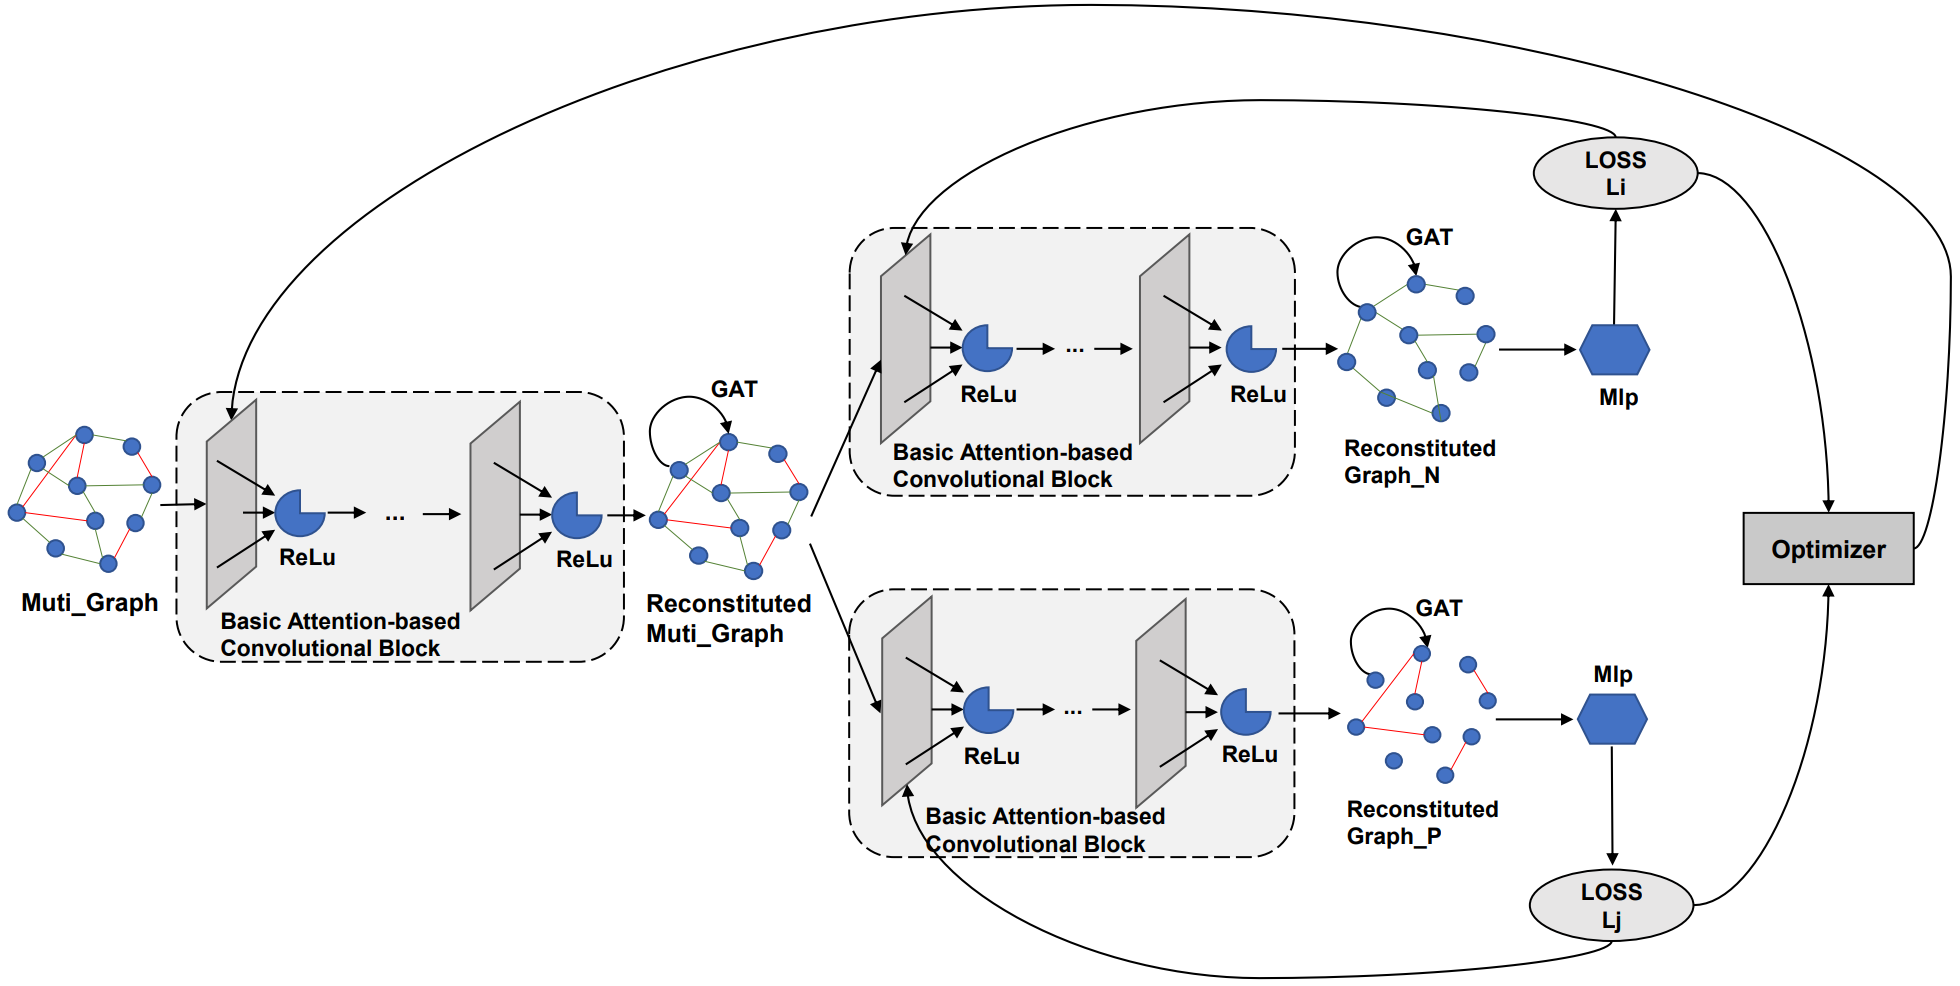
\includegraphics[width=1\textwidth]{img/跨域表示学习的总体框架.png}
    \caption{跨域表示学习的总体框架}
    \label{figure:跨域表示学习的总体框架}
\end{figure}

\subsection{多图构建}

在该方法中,目标是从ICS的多个域(如物理域、网络域等)中提取节点特征,并构建统一的多图结构用于跨域建模。
多图表示结构的构构建过程如\cref{figure:多图表示结构的构建过程}所示。

\begin{figure}[ht]
    \centering
    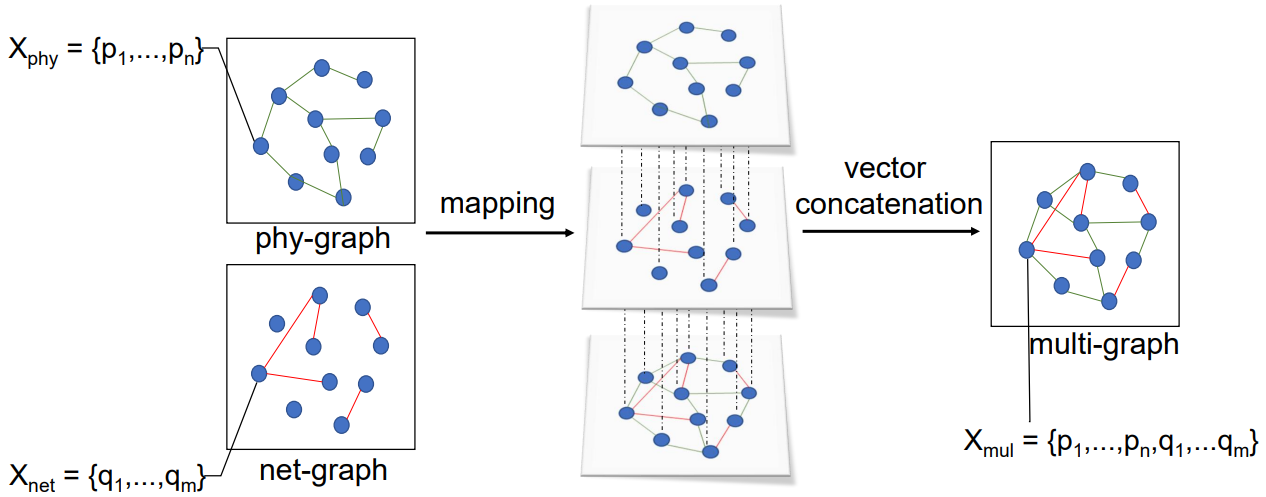
\includegraphics[width=1\textwidth]{img/多图表示结构的构建过程.png}
    \caption{多图表示结构的构建过程}
    \label{figure:多图表示结构的构建过程}
\end{figure}

假设有$n$个节点(传感器和执行器),来自不同域的数据被统一为相同的时间粒度(如秒级粒度),每个节点在第$d$个域上的特征矩阵为
\begin{equation*}
    \bm{x}^{(d)}\in\mathbb{R}^{n\times t} \text{,}
\end{equation*}
其中$t$为时间步长。

对每个域$d\in\{1,2,\cdots,D\}$, 构建一个无向加权图
\begin{equation*}
    \mathcal{G}_d=\left<\mathcal{V},\mathcal{E}_d\right> \text{,}
\end{equation*}
其中$\mathcal{V}$表示所有节点的集合,且$|\mathcal{V}|=n$,$\mathcal{E}_d$为第$d$个域中的边集合。

节点之间的边权通过余弦相似度计算其嵌入向量之间的相似性。
对于任意两个节点$i$和节点$j$,在第$d$域的嵌入向量为$\bm{v}_i^{(d)}$和$\bm{v}_j^{(d)}$,则计算节点$i$到节点$j$的边权
\begin{equation*}
    e_{ij}^{(d)}=\frac{\left(\bm{v}_i^{(d)}\right)^\mathrm{T}\bm{v}_j^{(d)}}{\left\|\bm{v}_i^{(d)}\right\|\left\|\bm{v}_j^{(d)}\right\|} \text{,}
\end{equation*}
之后使用Top-k策略筛选每个节点最相关的$k$个邻居构建图$\mathcal{G}_d$,进一步融合成多图结构
\begin{equation*}
    \mathcal{G}=\left<\mathcal{V}, \textstyle\bigcup_{i=1}^d\mathcal{E}_i\right> \text{,}
\end{equation*}
节点$i$的跨域特征向量表示为
\begin{equation*}
    \bm{v}_i=\bm{v}_i^{(1)}\oplus\bm{v}_i^{(2)}\oplus\cdots\oplus\bm{v}_i^{(D)} \text{。}
\end{equation*}

\subsection{基于注意力机制的图卷积神经网络建模}

文章引入GDN中的图注意力机制(Graph Attention Network, GAT)\cite{velickovic2018graph}对节点信息进行聚合,捕捉局部邻居中的非均匀关系。

首先,定义节点$j$对节点$i$的注意力权重
\begin{equation*}
    \alpha_{ij}=\mathrm{Softmax}\left(\mathrm{LeakeyReLU}\left(\bm{a}^\mathrm{T}(\bm{v}_i\oplus\bm{v}_j)\right)\right) \text{,}
\end{equation*}
其中$\bm{a}$为可学习的向量。则节点$i$的聚合表示更新为
\begin{equation*}
    \bm{z}_i=\mathrm{ReLU}\left(\alpha_{ii}\bm{W}\bm{v}_i+\bm{W}\sum_{j\in\mathcal{N}_i}\alpha_{ij}\bm{v}_j\right) \text{,}
\end{equation*}
其中$\bm{W}$为可学习的矩阵。

\subsection{融合输出}

使用节点的聚合表示和特征向量进行输出,即
\begin{equation*}
    \hat{\bm{y}}=f_\theta([\bm{z}_1\circ\bm{v}_1, \bm{z}_2\circ\bm{v}_2, \cdots, \bm{z}_n\circ\bm{v}_n]) \text{,}
\end{equation*}
其中$\circ$为逐元素乘法,$f_\theta$为多层感知机。
